\documentclass[a4paper, 12pt]{article}

\usepackage{amsmath, amsthm, amssymb, bm}
\usepackage{geometry}
\geometry{left=2.0cm,right=2.0cm,top=2.5cm,bottom=2.5cm}
\usepackage{graphicx}
\usepackage{color}
\usepackage{graphicx}
\usepackage{tikz}
\usetikzlibrary{automata,shapes.geometric}
\usepackage{array}
\usepackage{indentfirst}
\usepackage{float}

 \usepackage{multicol}
% \setlength{\columnsep}{0.7cm}
\usepackage{multirow}
\newcommand{\cbra}[1]{\left\{ #1 \right\}}
\newcommand{\bkm}[1]{{\color{cyan} #1}}
\newcommand{\pbra}[1]{\left( #1 \right)}


\begin{document}
\thispagestyle{empty}

\noindent Dear Editors,

\medskip 
\noindent We are delighted to present our manuscript titled \textbf{``Adaptive-depth randomized measurement for fermionic observables"} for your esteemed consideration for publication in the ``Quantum Science and Technology". 

\vspace{8pt}
\noindent \textbf{Background} \ \ Estimating properties of fermionic systems is an important problem in quantum information theory and quantum computing since it captures the intricacies of electron correlations and dynamics. The fermionic classical shadow (FCS) algorithm is introduced to efficiently predict many properties, such as the ground state energy, in a fermionic system. However, studies suggest that it requires a random measurement circuit with $\mathcal{O}(n^2)$ size quantum circuit, which exceeds the capabilities of current quantum devices. An intriguing open question remains: 
\emph{Is there an efficient shallow-depth FCS algorithm for specific sets of fermionic observables?}

\vspace{8pt}
\noindent \textbf{Main results} \ \ 
We propose an adaptive-depth fermionic classical shadow (ADFCS) protocol that reduces the depth requirements of FCS while preserving the measurement efficiency. Through theoretical analysis and numerical fitting, we demonstrate that the required depth for approximating a fermionic observable $H$ can be upper bounded by $\mathcal{O}\pbra{\max\cbra{\frac{d_{\text{int}}(H)^2}{\log n}, d_{\text{int}}(H)}}$, where $d_{\text{int}}(H)$ denotes the interaction distance of $H$, as detailed in the manuscript. Numerical results demonstrate that the ADFCS algorithm achieves comparable estimation accuracy while requiring shallower circuit depths for fermionic observables with small interaction distances. The following figure illustrates this comparison by presenting the estimation error for the expectation values of the Kitaev chain Hamiltonian using the ADFCS and FCS algorithms.
%We derive the relation between the depth and the sample complexity for $k$-local Fermionic observables for constant $k$.
%defined as the product of $k$ Majorana operators. 
%By setting the $k$ as a constant number, we investigate the optimal depth $d^\ast$ of the brickwork random circuit. The optimal depth $d^\ast$ is the minimum depth that keeps the sample complexity scales polynomially. We propose the adaptive-depth fermionic classical shadow (ADFCS) algorithm, which adaptively selects the optimal depth for a set of Majorana operators. We test the ADFCS algorithm on the Kiteav chain Hamiltonian and various Majorana operators. 


 % ADFCS estimates the properties of fermionic observables unbiasedly with a shallower depth, and it is efficient for k-local Majorana operators with constant k. This limitation is not narrow because k-local Majorana operators with constant k express the most interesting fermionic observables. The ADFCS algorithm's main idea is to adaptively select the depth $d^\ast$ of the random circuit.  The optimal depth $d^\ast$ is the minimum depth, which promises that the sample complexity scales polynomially. We also give the optimal depth order, which depends on the interaction distance of Majorana observables.

\begin{multicols}{2}
% \vskip 8pt
% \textbf{Significance}
\paragraph{Significance}
Our work offers the first insight into the capabilities of the FCS protocol using shallow-depth random matchgate circuits. We introduce an ADFCS measurement protocol that correlates with the interaction distance of the fermionic observable $H$, offering a novel approach to estimating fermionic properties. The algorithm can be applied to a broad range of quantum simulation approaches like VQE. This advancement is poised to significantly impact the learning fermionic Hamiltonians, paving the way for more efficient quantum simulations.



%\vspace{8pt}
% Our work gives a new understanding of the behavior of brickwork random matchgate circuits with varying depths. Moreover, the ADFCS algorithm reduces the cost of the quantum resource by adaptively selecting the depth, which offers a viable solution for near-term quantum devices. 
% We find an algorithm for estimating a set of Majorana observables with shallower depth compared with FCS, especially when the interaction distance of Majorana observables is small. Fortunately, 
% The interaction distance of most physical fermionic observables is $\mathcal{O}(\log n)$, such as the Ising model and Kiteav chain. It suggests that the expectation value of these observables can be estimated via a $\mathcal{O}(\log n)$ depth random circuit in ADFCS rather than a $\Omega(n^2)$ depth circuit in FCS. Thus, the ADFCS algorithm 
%\noindent Recognizing the substantial impact our research could deliver in the field of quantum information,
%we believe that our work is of broad interest to the readers of npj Quantum Information.
\columnbreak
\begin{figure}[H]
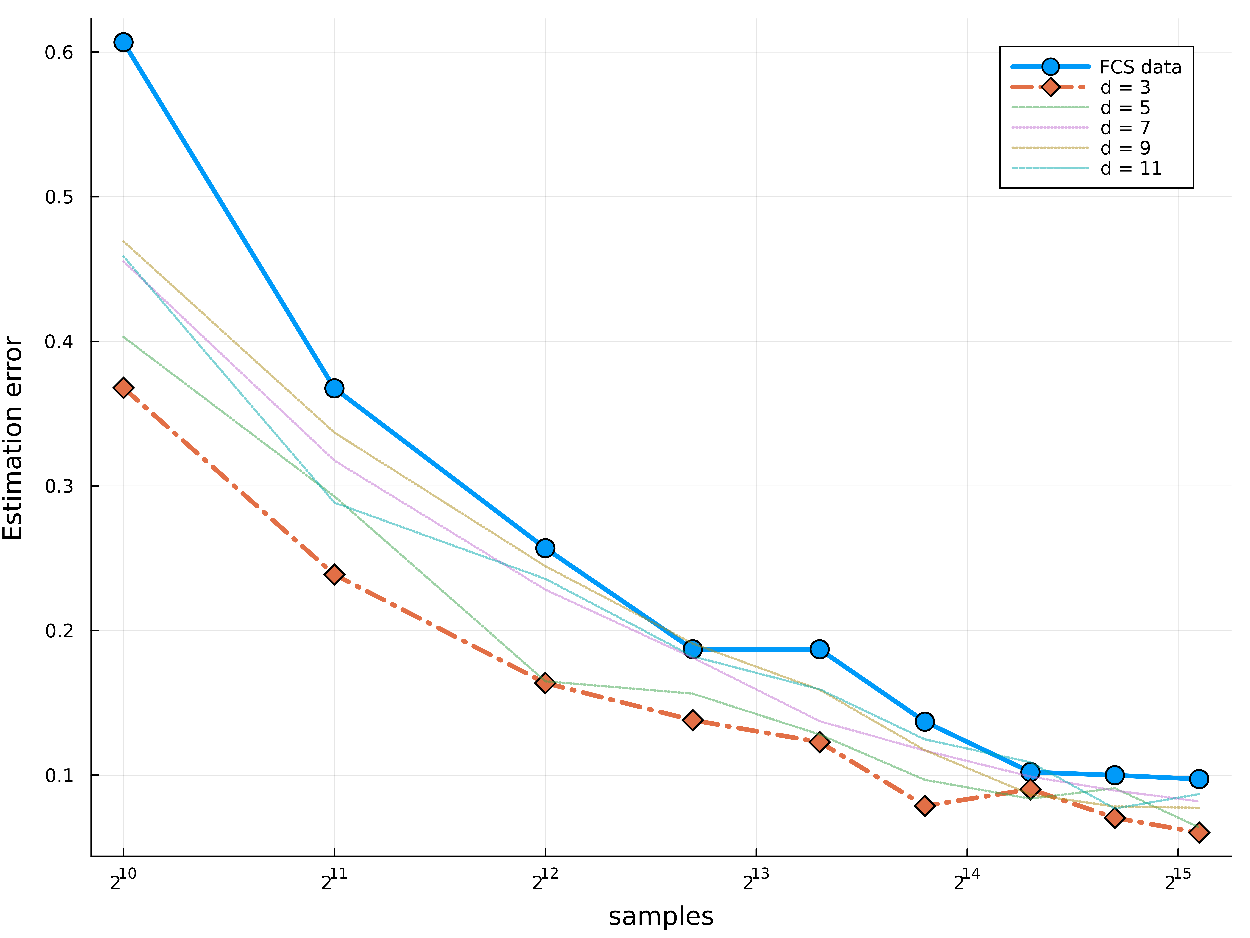
\includegraphics[width = 0.5\textwidth]{error_H.pdf}
\label{fig:Majorana}
\end{figure}
\end{multicols}

\noindent Recognizing the substantial impact our research could deliver in the field of quantum information and computation, we believe that our work is of broad interest to ``Quantum Science and Technology" readers.

\vspace{8pt}
\noindent Thank you very much for your time and consideration.

\vspace{8pt}
\noindent  Yours sincerely, 

\noindent Kaiming Bian and Bujiao Wu.

% \noindent \textbf{Corresponding authors:}
% \begin{itemize}
%     \item Kaiming Bian \\ 
%     Affiliation: Shenzhen Institute for Quantum Science and Engineering,
% Southern University of Science and Technology, Shenzhen 518055, China; \& International Quantum Academy, Shenzhen 518048, China; \& Guangdong Provincial Key Laboratory of Quantum Science and Engineering, Southern University of Science and Technology, Shenzhen, 518055, China. \\
% Phone numbers: +86-13860654482 \\ 
% E-mail address: 12231295@mail.sustech.edu.cn
%     \item Bujiao Wu \\
%     Affiliation: Shenzhen Institute for Quantum Science and Engineering,
% Southern University of Science and Technology, Shenzhen 518055, China; \& International Quantum Academy, Shenzhen 518048, China; \& Guangdong Provincial Key Laboratory of Quantum Science and Engineering, Southern University of Science and Technology, Shenzhen, 518055, China. \\
% Phone numbers: +86-18813177880 \\
% E-mail address: bujiaowu@gmail.com
% \end{itemize}

% \noindent \textbf{Conflict of interest statement for all authors:}
% The authors declare that they have no conflict of interest.

% \newpage 

% \vspace{8pt}
% \noindent \textbf{Suggested reviewers:}
% \begin{itemize}
%     \item Daniel Miller; Free University Berlin; \\
%     d.miller@fu-berlin.de
%     \item Andrew Zhao; Sandia National Laboratories, California, United States \\
%     andrew.zhao@sandia.gov  
    
%     \item You Zhou; Key Laboratory for Information Science of Electromagnetic Waves (Ministry of Education), Fudan University, Shanghai 200433, China; \\
%     you\_zhou@fudan.edu.cn

%     \item Antonio Anna Mele; Free University Berlin;\\
%     mele@fu-berlin.de

%     \item Xiongfeng Ma; Center for Quantum Information, Institute for Interdisciplinary Information Sciences, Tsinghua University, Beijing 100084, P. R. China;\\
%     xma@tsinghua.edu.cn

%     \item Christian Bertoni; Free University Berlin; \\
%     bertoni@zedat.fu-berlin.de
    
%         \item Guang Hao Low; Microsoft Quantum, Redmond, Washington 98052, USA; \\
%     GuangHao.Low@microsoft.com

% \end{itemize}


% \vspace{8pt}
% \noindent \textbf{Background} \ \ Estimating properties of fermionic systems is one of the most important problems in quantum computing and quantum information since it captures the intricacies of electron correlations and dynamics. The fermionic classical shadow (FCS) algorithm is introduced to efficiently predict many properties in a fermionic system. However, studies suggest that it requires a random measurement circuit with $\mathcal{O}(n^2)$ size quantum circuit, which exceeds the capabilities of current quantum devices. An intriguing open question remains: 
% \emph{Is there an efficient shallow-depth FCS algorithm for specific sets of fermionic observables?}

% \vspace{8pt}
% \noindent \textbf{Main results} \ \ 
% We propose an adaptive-depth fermionic classical shadow (ADFCS) protocol that reduces the depth requirements of FCS while maintaining the required measurements. Through theoretical analysis and numerical fitting, we demonstrate that the required depth for approximating a fermionic observable $H$ scales linearly with $\max\cbra{\frac{d_{\text{int}}(H)^2}{\log n}, d_{\text{int}}(H)}$, where $d_{\text{int}}(H)$ denotes the interaction distance of $H$, as detailed in the manuscript. Numerical results demonstrate that the ADFCS algorithm achieves comparable estimation accuracy while requiring shallower circuit depths for fermionic observables with small interaction distances. The following figure illustrates this comparison by presenting the estimation error for the expectation values of the Kitaev chain Hamiltonian using the ADFCS and FCS algorithms.


% \begin{multicols}{2}
% % \vskip 8pt
% % \textbf{Significance}
% \paragraph{Significance}
% Our work offers the first insight into the capabilities of the FCS protocol using shallow-depth random matchgate circuits. We introduce an ADFCS measurement protocol that correlates with the interaction distance of the fermionic observable $H$, offering a novel approach to estimating fermionic properties. This advancement is poised to significantly impact the learning of physical and chemical Hamiltonians, paving the way for more efficient quantum simulations.





\end{document}